\acresetall
\chapter{Learning and Memory}
\label{ch:intro:memory}
\section*{Overview}
Learning and memory define who we are and shape who we will become.
The various components of memory -- learning, adaptation, plasticity, association, conditioning -- are fundamental features of nervous systems across all organisms.
Indeed, humanity's greatest adaptation is perhaps our unparalleled ability to learn from and adapt to the world around us.
The study of memory in the brain spans from the level of molecular changes that occur at the synapse between individual cells to the role of entire brain regions in facilitating different components of memory.
% Over time, our understanding of memory has evolved from the earliest quantifications of the limits of human memory \citep{Ebbinghaus1885} to a molecular understanding of the changes within the brain that occur following learning \citep{Kandel2001}.

In the following sections I aim to describe an understanding of memory, the brain structures underlying it, and cellular physiological correlates of learning relevant to my later studies.
In discussing learning and memory, I will first focus on spatial memory as a core component of episodic memory (\ref{sec:intro:memory:memory}) and how we experimentally study it.
While learning-related changes are fundamental to every neuron in the nervous system, I will primarily focus on the role of the \ac{HPC} in learning and memory, as the \ac{HPC} is most relevant to the memory systems I will be studying (\ref{sec:intro:memory:structure}).
Finally, I will discuss our current understanding of cellular and circuit mechanisms by which the brain encodes and recalls memory, with a specific emphasis on hippocampal place cells underlying spatial memory (\ref{sec:intro:memory:physiology}).

\section{Memory}\label{sec:intro:memory:memory}
Memory is the way in which experiences from the past can influence how we interpret the present (or the future).
Memory includes both explicit memories of objects, concepts, people, places, and events (\textsc{declarative memory}), but also skills and abilities that we cannot consciously recall, such as the ability to shoot a basketball or improve painting skills with practice (\textsc{implicit memory}).
Forms of implicit memory are evolutionarily ancient, present in the earliest invertebrates \citep{Milner1998}.

Declarative memory can be subdivided into at least two categories: autobiographical episodic memory of events and semantic memory, which is the general knowledge of facts.
As Endel Tulving explained when he defined \textsc{episodic memory}, these two memory systems are not entirely independent:

% Episodic memory is 
% Episodic memory \citep{Tulving1972}
% Ebbinghaus H (1885). Über das Gedachtnis, Dunker & Humbolt.
% https://books.google.com/books?id=kfA0AAAAMAAJ&ots=hjMhksDE3X&dq=Ebbinghaus%20H%20(1885).%20%C3%9Cber%20das%20Gedachtnis%2C&lr&pg=PA1#v=onepage&q&f=false

\begin{quote}
Episodic memory retrieves and stores information about temporally dated episodes or events, and temporal-spatial relations among these events. A perceptual event can be stored in the episodic system solely in terms of its perceptible properties or attributes, and it is always stored in terms of its autobiographical reference to the already existing contents of the episodic memory store. The act of retrieval of information from the episodic memory store, in addition to making the retrieved contents accessible to inspection, also serves as a special type input into episodic memory and thus changes the contents of the episodic memory store. The system is probably quite susceptible to transformation and loss of information. While the specific form in which perceptual input is registered into the episodic memory can at times be strongly influenced by information in semantic memory -- we refer to the phenomenon as encoding -- it is also possible for the episodic system to operate relatively independently of the semantic system.
\attrib{\citealt[pgs.~385-386]{Tulving1972}}
\end{quote}

My work is primarily concerned with...
\todo[color=green]{This needs to be a bit more cohesive and flow better}

% \begin{quote}
% Consider now a typical memory experiment in which a subject is asked to study and remember a list of familiar words or pair of words. This is an episodic memory task. The occurrence of a verbal item in a given list, at a particular time, and in specific temporal relation to other items in the list is an autobiographical episode having no necessary extra-episodic denotative reference. The subject has successfully retrieved information about this episode when he responds to the retrieval query with the reproduction if an appropriate copy of the input item.
% \attrib{\citealt{Tulving1972}}
% \end{quote}

% \begin{quote}
% Each experienced event always occurs at a particular spatial location and in a particular temporal relation to other events that already have occurred, events occurring simultaneously with it, or events that have not yet occurred. These temporal relations among experienced events are also somehow represented as properties of items in the episodic memory system. To ask a person about some item in episodic memory means to ask them when did event $E$ happen, or what events happened at time $T$. Retrieval of information of this kind from episodic memory is successful if the person can describe the perceptible properties of the event in question and more or less accurately specify its temporal relations to other events. Temporal coordinates of an event and its representation in episodic memory of course need not be specified in terms of the clock and the calendar. They could be recorded in terms of temporal occurrences of other events in some as yet little understood manner.
% \attrib{\citealt[pg.~388]{Tulving1972}}
% \end{quote}

% Eichenbaum H, Yonelinas AR, Ranganath C (2007): The medial tempo- ral lobe and recognition memory. Annu Rev Neurosci 30:123–152.
% Milner B, Squire LR, Kandel ER (1998): Cognitive neuroscience and the study of memory. Neuron 20:445–468.
% 23.
% Fortin NJ, Wright SP, Eichenbaum H (2004): Recollection-like memory retrieval in rats is dependent on the hippocampus. Nature 431:188– 191.
% Sauvage MM, Fortin NJ, Owens CB, Yonelinas AP, Eichenbaum H (2008): Recognition memory: Opposite effects of hippocampal dam- age on recollection and familiarity. Nat Neurosci 11:16–18.

\subsection{Spatial memory}\label{sec:intro:memory:spatial}
Spatial memory is the aspect of our memory that instills our sense of direction and allows us to know where we are at any given time (our personal `GPS'), imagine or plan where we will be in the future, and know where we were when we recall particular memories.


Spatial navigation consists of two primary components: location relative to an allocentric map of the world, and egocentric update cues arising from orientation and other vestibular input.
The dominance of allocentric or egocentric navigation depends upon the precise nature of the environment being explored; egocentric dominates in cue-rich environments, while allocentric navigation dominates when landmarks are lacking or in the dark \citep{Knierim1998}\todo[color=green]{ref place cells in the dark paper}.

Spatial memory has been studied extensively in rodents, in large part because it a well-defined and tractable area of research.
As rodents can not be asked to recall past events, we need assays that can probe for evidence of these memories (\nameref{sec:intro:memory:spatial-reward}).
Not only do we have good behavioral tests for spatial memory in rodents, but we have identified the cognitive map of the memory itself (\nameref{ec:intro:memory:spatial_maps}).
% Allocentric navigation in particular is \ac{HPC}-dependent \citep{OKeefe1978, Smith1989}, not egocentric.

\subsubsection{Spatial memory as episodic memory}\label{sec:intro:memory:spatial-episodic}
% In 1972 Endel Tulving coined the term \textsc{episodic memory}, describing it as follows:

% \begin{quote}
% Episodic memory retrieves and stores information about temporally dated episodes or events, and temporal-spatial relations among these events...Each experienced event always occurs at a particular spatial location and in a particular temporal relation to other events that already have occurred, events occurring simultaneously with it, or events that have not yet occurred.
% \attrib{\citealt{Tulving1972}}
% \end{quote}

Experiences are innately inseparable from the time and place at which they occurred.
When we think of an autobiographical memory, we remember the experience (e.g. waiting in line to get lunch) along with the location (e.g. Mike's Bagels at 168\super{th} and Broadway) and the time (e.g. last Tuesday around 2PM) they occurred.
This applies to psychological memory tests as well, such as remembering words on a list, where the temporal order of items on the list (I saw `orange' before `banana') and the visio-spatial arrangement of the words on the paper list (`boat' was written above `car') are core components of the stored memory.
Even more than being a component of episodic memory, spatial memory may in fact \emph{be} episodic memory.
The brain structure most closely associated with episodic memory (\nameref{sec:intro:memory:hpc}) has also shown to contain cells which directly map to real world locations (\nameref{sec:intro:memory:spatial_maps}).
Indeed it has been proposed that the same neural mechanisms may underly both the ability to store the relationship amongst objects in a remembered experience, and the relationship between landmarks contributing to a map of space \citep{Buzsaki2013}.

\subsection{Spatial reward learning}\label{sec:intro:memory:spatial-reward}
Tests of spatial memory are fundamental tools for rodent researchers, and a particular focus of my thesis work.
The most widely used assay of spatial memory is the \textsc{Morris water maze} \citep{Morris1984}.
While there is variability in the details of the protocol, the general structure is usually the same.
Briefly, the `maze' is a large water-filled tub with a single hidden platform under the surface of the water.
Mice or rats are placed in the maze and over successive trials eventually learn to use distal cues around the room to locate the platform.
Probe trials generally consist of removing the platform and scoring the fraction of time spent in the correct quadrant as a measure of spatial memory.
More recently, virtual reality variations of the Morris water maze have been developed that allow for head-fixed spatial learning tasks in rodents \citep{Aronov2014} or the ability to mirror rodent experimental paradigms in humans \citep{}.
Virtual reality water mazes have been to study spatial memory in \scz/ patients, which I will discuss later (\autoref{sec:intro:scz:spatial}).

One particular variation is the annular water maze used by \citeauthor{Hollup2001a}, which adds an inner wall to the large circular pool creating a `one-dimensional' circular track that the mice swim around.
This task is similar to the \ac{GOL} task (\autoref{sec:intro:techniques:GOL}) that I use throughout my primary experiments; both tasks require rodents to find hidden rewards in a simplified `one-dimensional' environment while recording from hippocampal area CA1 pyramidal cells and quantify both the task performance and place cell enrichment of the reward location.
In particular, the authors find an accumulation of place cells around the escape platform (\autoref{fig:intro:memory:hollup}), a finding which I replicate and expand upon in my \ac{GOL} task (\autoref{sec:df:results:enrichment}). 
\begin{figure}
	\centering
	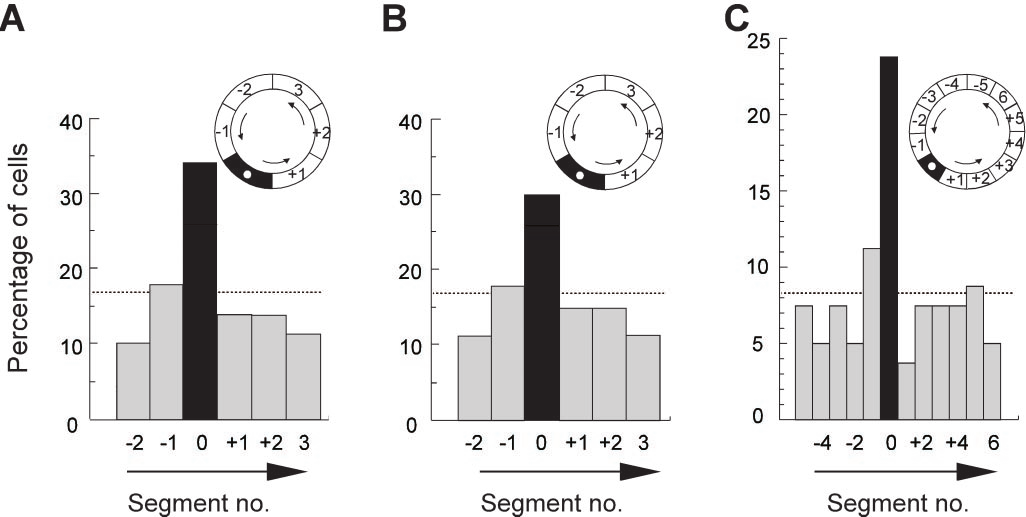
\includegraphics[width=0.7\textwidth]{intro/Hollup_accumulation}
	\caption[Distribution of firing fields from Hollup et al.]{Distribution of firing fields after training with a constant platform location.
	(A) Percentage of firing fields in each 60$^{\circ}$ segment of the corridor (80 cells; average of 3 probe tests). Field location was defined as the segment with the maximal averaged firing rate. Firing fields accumulated in the platform segment (segment 0, black). The chance level was at 16.7\%. Inset, Diagram of the corridor. Arrows indicate swim direction.
	(B) Percentage of firing fields in each 60$^{\circ}$ segment after directional sorting (same trials and same symbols as described in A). Only data sampled during swimming in the preferred direction are retained.
	(C) Percentage of firing fields in segments of 30$^{\circ}$ after directional sorting. The platform was in the middle of segment 0.
	Reproduced from \citet{Hollup2001a}.}
	\label{fig:intro:memory:hollup}
\end{figure}

Conceptually similar, but drier, are the Barnes or cheeseboard maze \citep{Barnes1979}\citep{Kesner1991}\citep{Dupret2010a}.
These mazes consist of a large platform with holes throughout.
These holes can either be escapes for the mice/rats to avoid the exposed platform, or baited/rewarded.
Either way, the degree of learning can be quantified by latency to finding the correct location or time spent near previously rewarded locations during un-rewarded probe trials.
In a study by \citeauthor{Dupret2010a} which partially inspired my own work, the authors used a cheeseboard maze to examine hippocampal functional correlates of learning and memory (see \autoref{sec:df:methods:comp}).
They authors identified an increase in the fraction of hippocampal area CA1 place cells that encoded the reward location, the magnitude of which correlated with task performance (\autoref{fig:intro:memory:dupret}a,b).
In addition they found properties of sharp-wave ripples (SWRs) that also correlated with task performance -- the fraction of pyramidal cells that participated in sharp-wave ripple events during exploration (eSWRs) and the similarity of the pyramidal cell firing patterns during off-line SWRs (sSWRs) with on-line exploration of the reward locations (\autoref{fig:intro:memory:dupret}c,d).
In light of evidence pointing to a central role for SWRs in long-term memory consolidation \citep{Buzsaki2015}, it's tempting to interpret these findings as task performance being aided by an increased number of pyramidal cells encoding a memory of the reward locations during exploration and increased `remembering' of the rewarded locations during sleep.
In my own experiments, we found dysfunctional SWR activity in mice that performed worse on our similar \ac{GOL} task, which aligns with these results (\autoref{sec:df:results:SWR}).

\begin{figure}
	\centering
	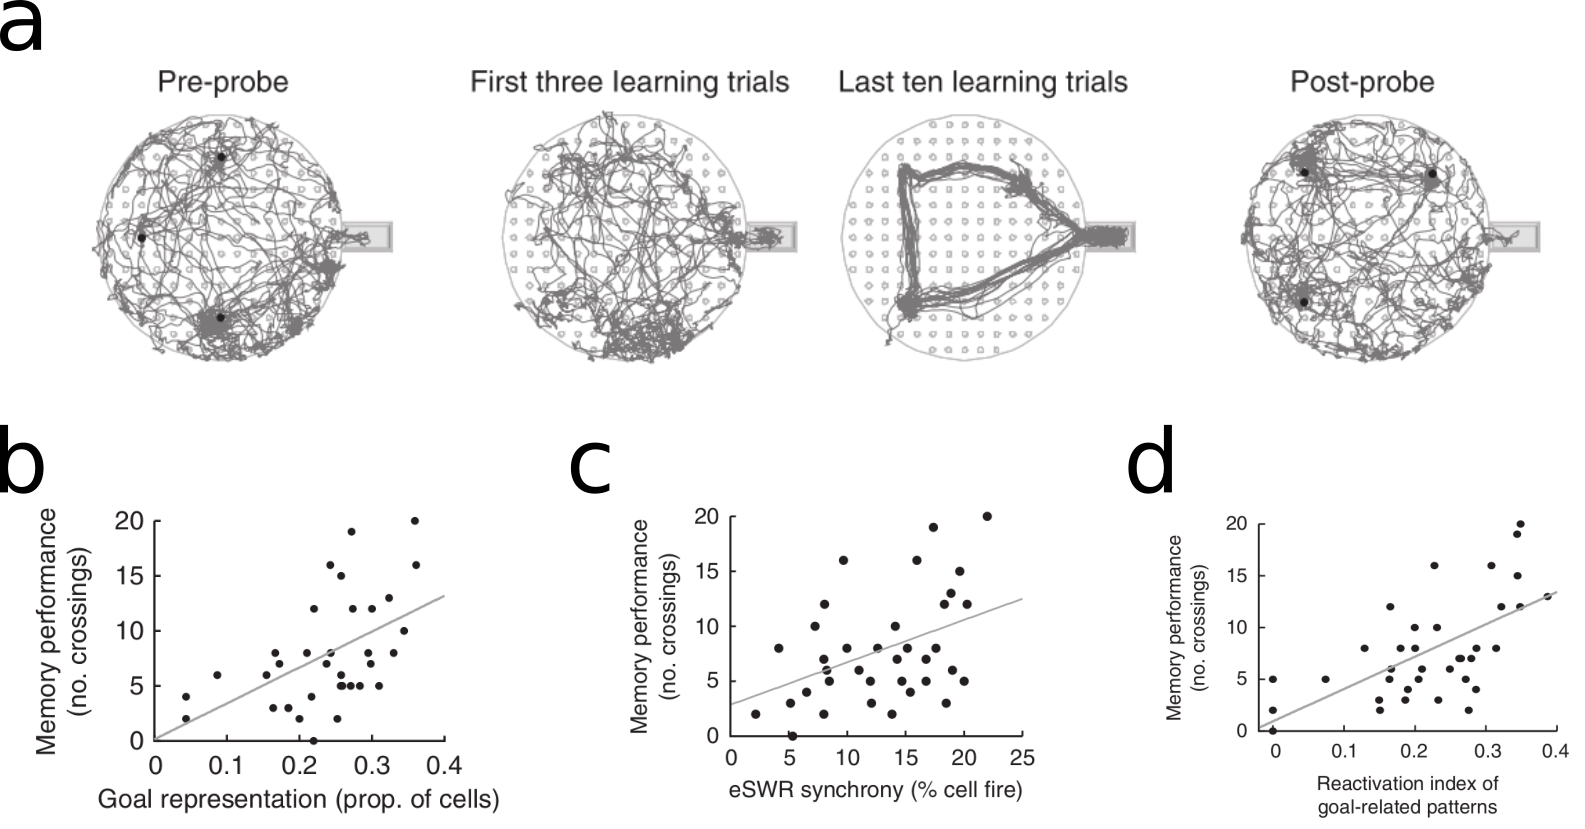
\includegraphics[width=0.7\textwidth]{intro/Dupret_cheeseboard_and_correlates}
	\caption[Cheeseboard task and behavioral correlates from Dupret et al.]{Cheeseboard task and behavioral correlates from Dupret et al.
	(a) Representative examples of an animal's path; for clarity, only the first 10 min of each probe session is depicted (black dots, learnt goal locations).
	(b) Scatter plot showing post-probe memory performance (number of crossings) as a function of the proportion of CA1 place cells at goal location during the end of learning (gray: regression line, r~=~0.511, P=0.0014).
	(c) Scatter plot showing post-probe memory performance (number of crossings) as a function of `eSWR synchrony' (percentage of CA1 pyramidal cells that fire in eSWR) at the end of learning (gray: regression line, r~=~0.418, P=0.011).
	(d) Scatter plot showing post-probe memory performance (number of crossings at a given goal location) as a function of the proportion of sSWRs in which assembly patterns represented the same goal location (gray: regression line, r~=~0.620, P=0.00005)
	Figures rearranged and reproduced from \citet{Dupret2010a}.}
	\label{fig:intro:memory:dupret}
\end{figure}

\section{Memory in the brain}\label{sec:intro:memory:structure}
The earliest behaviorist approaches to studying memory focused solely on the behavioral responses elicited by sensory inputs -- ignoring the `black box' that was the brain at the time. \todo[color=green]{behaviorist reference?}
Since then, it is now, perhaps obviously, recognized that behavioral responses intimately depend upon the source of the response -- the brain.
The degree to which memory, and more generally cognitive functions, are localized within the brain has been widely debated.
In the late 1800's Pierre Paul Broca and Carl Wernicke identified patients with specific speech deficits related to the production and comprehension of language respectively.
These deficits were later found to be associated with specific lesions in the posterior inferior frontal gyrus and posterior section of the superior temporal gyrus, providing evidence for the localization of cognitive functions within the brain.
In contrast, work by Karl Lashley in the early 20\super{th} century showed that following the systematic removal of pieces of rat neocortex, performance in a previously-learned maze depended on the size of the lesions, but not the specific location \citep{Lashley1929}, lending support for the alternate \textsc{theory of mass action}.
Donald Hebb was one of the first to bring these two theories together, suggesting that networks of neurons could span many brain regions and collectively store memories \citep{Hebb1949}.
There are clearly cognitive functions that are localized to specific regions of the brain, but none of these function independently, and circuits that perform specific computations span the entire brain.\todo[color=green]{rewrite this sentence}

While `memory' in it's broadest sense is a fundamental feature of every neuron, in mammals certain memory sub-types have been closely associated to specific brain regions.
For example, implicit \textsc{procedural memory} (\todo[color=green]{procedural memory example}) is largely localized to the \textsc{striatum} and \textsc{cerebellum} \todo[color=green]{procedural memory reference}, while \textsc{emotional memory}, such as fear, is largely attributed to the \textsc{amygdala} \citep{LeDoux2000}.
The \textsc{neocortex} is important for \textsc{working memory}, \textsc{priming} effects, and eventually the long-term storage of \textsc{declarative memory}.
While declarative memory may eventually be store in the cortex, the \ac{HPC} is central to the process of consolidating declarative memories of experiences, and building association networks, such as in the case of spatial maps \citep{Eichenbaum2000}.
My primary research focus revolved around hippocampal-dependent spatial memory, so with no desire to minimize the important role of the rest of the brain in memory, I will focus on the \ac{HPC} for the remainder of this section. 

\subsection{The Hippocampus}\label{sec:intro:memory:hpc}
The \ac{HPC} has been central to our study of memory at least since Scoville and Milner first reported in the 1950's on Henry Molaison (H.M.) who had profound anterograde amnesia following the bilateral removal of large portions of the medial temporal lobes, which includes the \ac{HPC} and parahippocampal structures \citep{Scoville1957}.
The most dramatic feature of H.M.'s memory loss was the inability to form new episodic memories, as he described it:
\begin{quote}
Every day is alone in itself, whatever enjoyment I've had, and whatever sorrow I've had.
\attrib{in \citealt{Milner1968}}
\end{quote}
Despite H.M.'s near complete inability to form new memories, he still maintained the ability to recall events from childhood and showed no general cognitive or intelligence decline \citep{Squire2009}.
% lending evidence to the idea of a distributed memory system, or at least separable facets of memory .
Additional studies of H.M. over the next 50 years revealed that while declarative memory deficits remained severely impaired, various forms of implicit memory remained unaffected \citep{Corkin2002}.
For example, patient H.M. was able to show day-to-day improvements in a mirror-tracing motor-learning task, despite no explicit memory of ever having performed the task before.
In addition, he showed normal word-list priming effects -- whereby words stems are preferentially completed by words semantically similar to recently viewed words. 
While the specific brain areas resectioned in the case of H.M. included structures adjacent to the \ac{HPC} as well (such as the amygdala), numerous studies have since shown that the \ac{HPC} in particular is essential for normal formation of long term episodic and semantic memory \citep[reviewd in][]{Eichenbaum2000, Burgess2002}.

CA2 social memory \\
DG pattern separation \\
CA3 pattern completion \\
CA1 comparator/contextual integration \\
spatial memory \\
association networks \\
environment/context coding

\subsubsection{Dorsal vs. lateral HPC}
The \ac{HPC}
\todo[inline, color=red]{Dorsal vs. lateral HPC}
\citep{Strange2014}
Dorsal is spatial, ventral is emotion, social
\subsubsection{Circuitry}
The \ac{HPC} is one of the most well-characterized neuronal circuits within the mammalian brain.
The principal neurons in the \ac{HPC} communicate through the classically-defined trisynaptic loop: perforant path fibers project from layer II of the entorhinal cortex (EC) to granule cells in the dentate gyrus, which in turn send mossy fiber projections to CA3 that finally project along the Schaffer collateral pathway and synapse upon proximal apical and basal dendrites of CA1 pyramidal cells (CA1PCs), which are the primary output node of the \ac{HPC}.
Among other projections to both cortical and subcortical structures, CA1PCs also send a projection back to deep layers of the EC, completing the hippocampal loop.
In addition, layer II of EC sends a direct perforant path projection to CA3 and layer III sends a direct projection through the temporoammonic pathway to distal dendrites of CA1.
Large excitatory cells within the hilus (\textsc{mossy cells}) receive excitation from dentate gyrus granule cells and provide both direct feedback excitation and indirect feedback inhibition to granule cells.
There is also a long-range inhibitory projection (LRIP) from both medial and lateral entorhinal cortex that targets inhibitory interneurons -- which in turn target CA1PC tuft dendrites -- near the SR-SLM border in CA1, conveying spatial and contextual information respectively \citep{Basu2016}.
In \autoref{sec:other:LRIP}, I will discuss work I did characterizing the functional properties of the LRIP from LEC to CA1. 
% Stellate Ocean cells in ECII project to the DG, CA3, and CA2 region, whereas ECIII cells directly project to the CA1 region. % Entorhinal–hippocampal neuronal circuits bridge temporally discontiguous events, Tonegawa

% \begin{figure}
% 	\centering
% 	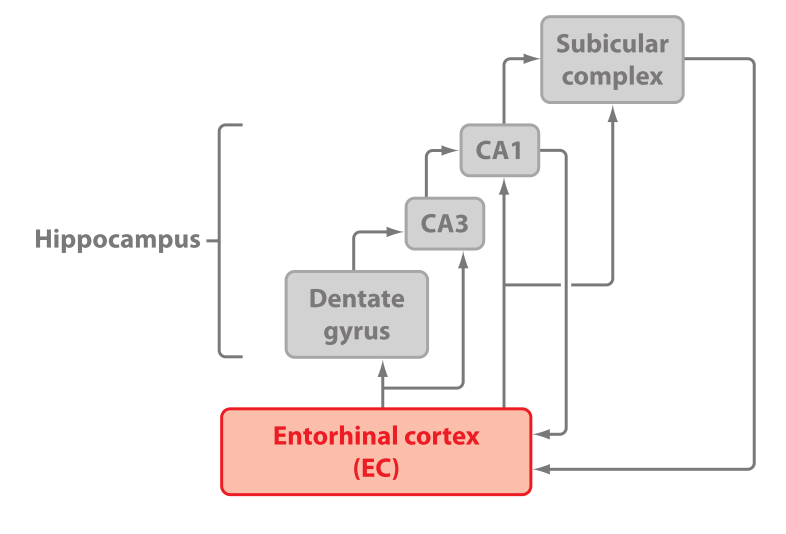
\includegraphics[width=0.5\textwidth]{intro/Squire2011_HPC_circuitry_edit}
% 	\caption[Schematic view of the medial temporal lobe memory system for declarative memory]{Schematic view of the medial temporal lobe memory system for declarative memory, which is composed of the hippocampus and the perirhinal, entorhinal, and parahippocampal cortices. In addition to the connections shown here, there are also weak projections from the perirhinal and parahippocampal cortices to the CA1-subiculum border.
% 	Reproduced from \citet{Squire2011}.}
% 	\label{fig:intro:memory:HPC_circuitry}
% \end{figure}
\begin{figure}
	\centering
	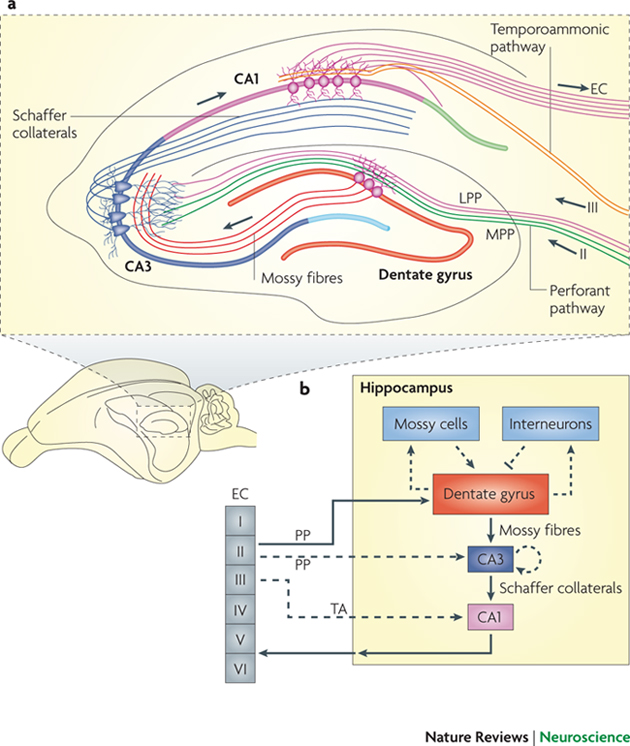
\includegraphics[width=0.7\textwidth]{intro/Deng2010_HPC_circuitry}
	\caption[The neural circuitry in the rodent hippocampus]{The neural circuitry in the rodent hippocampus.
	(a) An illustration of the hippocampal circuitry.
	(b) Diagram of the hippocampal neural network. The traditional excitatory trisynaptic pathway (entorhinal cortex (EC)--dentate gyrus--CA3--CA1--EC) is depicted by solid arrows. The axons of layer II neurons in the entorhinal cortex project to the dentate gyrus through the perforant pathway (PP), including the lateral perforant pathway (LPP) and medial perforant pathway (MPP). The dentate gyrus sends projections to the pyramidal cells in CA3 through mossy fibers. CA3 pyramidal neurons relay the information to CA1 pyramidal neurons through Schaffer collaterals. CA1 pyramidal neurons send back-projections into deep-layer neurons of the EC. CA3 also receives direct projections from EC layer II neurons through the PP. CA1 receives direct input from EC layer III neurons through the temporoammonic pathway (TA). The dentate granule cells also project to the mossy cells in the hilus and hilar interneurons, which send excitatory and inhibitory projections, respectively, back to the granule cells. 
	Reproduced from \citet{Deng2010}.}
	\label{fig:intro:memory:HPC_circuitry}
\end{figure}


Finally, the \ac{HPC} is targeted by afferents from neuromodulatory nuclei, including cholinergic and GABAergic projections from the medial septum  \citep{Klausberger2008}, serotonergic and glutamatergic projections from the raphe nuclei \citep{Varga2009}, as well as dopaminergic and noradrenergic projections from the ventral tegmental area \citep{Gasbarri1997} and locus coeruleus \citep{Foote1983}.
\todo[inline, color=yellow]{local IN in HPC}


% Burwell RD (2000): The parahippocampal region: Corticocortical connectivity. Ann N Y Acad Sci 911:25–42.
\subsubsection{CA1}
Pyramidal cells in hippocampal area CA1 are the principal excitatory neuron in that region and the primary output from the \ac{HPC}.
\todo[inline, color=red]{discuss CA1}
\todo[inline, color=yellow]{diversity in CA1PCs}
\begin{figure}
	\centering
	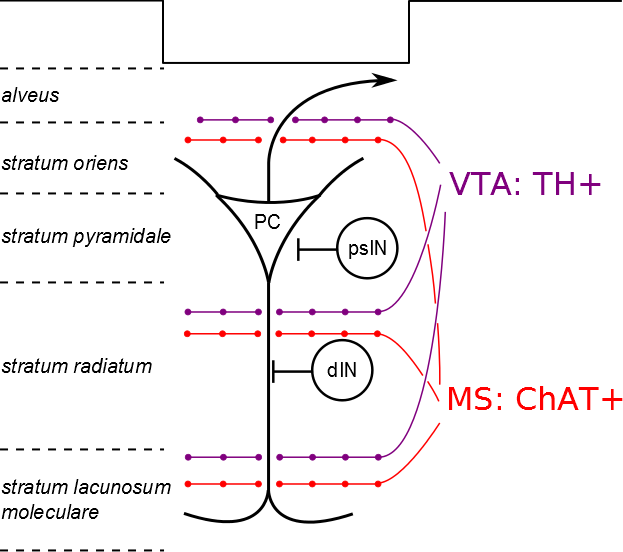
\includegraphics[width=0.5\textwidth]{intro/CA1-schematic_INs_VTA_MS}
	\caption{Schematic of major inputs to CA1 pyramidal cells}
	\label{fig:intro:memory:CA1_schematic}
\end{figure}


\subsection{Other}
In discussing the role of the \ac{HPC}, I've focused on spatial memory, but this is clearly not the sole role of the \ac{HPC}.
% \todo[inline]{Time cells}
\todo[inline, color=yellow]{LTP/conversion to longterm memory}
\todo[inline, color=yellow]{environment/context coding}
% \todo[inline]{pattern completion/separation}

\subsection{Memory at the synapse}
\todo[inline, color=red]{NMDAR/LTP}

\section{Functional correlates of memory}\label{sec:intro:memory:physiology}

\subsection{}

\subsection{Memory engrams}
\todo[color=yellow]{Memory engrams section?}

\subsection{Spatial maps}\label{sec:intro:memory:spatial_maps}
Perhaps the best-studied `engrams' in the mammalian brain are hippocampal place cells.
Throughout the \ac{HPC} (dentate gyrus, CA3, CA2, and CA1) there are principal cells that fire selectively at specific locations within an environment (\textsc{place cells}).
As an animal explores an environment these pyramidal cells show sparse spatially-modulated changes in firing rates that are established rapidly and subsequently remain stable \citep{O'Keefe1971}\citep{Thompson1990}\citep{Frank2004}.
These place cells form an allocentric map of the environment, which is essential for normal episodic memory function \citep{Smith2006c}\citep{Nakazawa2004}\citep{Buzsaki2013}.
Our understanding of place cells is a uniquely well-characterized functional mapping of the real world multiple synapses from both sensory and motor cortices.
Within the entorhinal cortex, principal cells take on a variety of spatial firing properties, but one of the main categories are cells that fire at regularly spaced intervals throughout an environment (\textsc{grid cells}) \citep{Hafting2005, Moser2014a}.
Place cells and grid cells together form the cellular foundation for the mammalian navigation system, and their discovery was recently awarded with the Nobel Prize in Medicine.

% \subsection{Place cells}\label{sec:intro:memory:place_cells}
\begin{figure}
	\centering
	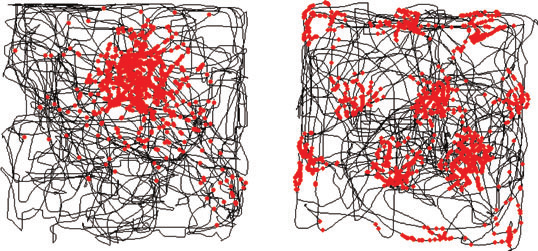
\includegraphics[width=0.7\textwidth]{intro/Moser_2008_place_grid}
	\caption[Place cell in the hippocampus and grid cell in the MEC]{Place cell in the hippocampus (a) and grid cell in the medial entorhinal cortex (MEC) (b).
	Spike locations (\emph{red}) are superimposed on the animal’s trajectory in the recording enclosure (\emph{black}).
	Whereas most place cells have a single firing location, the firing fields of a grid cell form a periodic triangular matrix tiling the entire environment available to the animal.
	Reproduced from \citet{Moser2008}.}
	\label{fig:intro:memory:place_grid}
\end{figure}

\subsubsection{Remapping}
Place cells, like other forms of memory, are constantly trying to balance two competing constraints: on the one hand, their firing needs to be stable in order to be a helpful representation of the environment, but on the other hand, their firing needs to be plastic enough to constantly encode new environments, forget irrelevant information, and adapt to new features.
Place cells changing their firing properties to incorporate new features of the world is known as \textsc{remapping} \citep{Muller1987}\citep{Leutgeb2005a}\citep{Colgin2008}.
A given place cell is defined by it's spatial tuning -- it's place field -- and it's firing rate gain within the place field.
These seem to be independent factors, as either can remap separately.
\textsc{Global remapping} is the collective remapping of place field locations across a population of place cells.
Alternatively, \textsc{rate remapping} is a change in place field gain (the ratio of firing rate in to out of the place field), while place fields locations remain fixed.

Global remapping is generally triggered by discrete changes to environmental conditions \citep{Leutgeb2004, Leutgeb2005a}, but can also be triggered by particularly salient events \citep{Moita2004}.
The sudden and collective remapping of firing fields support the notion of place fields arising from discrete attractor states \citep{Jeffery2011a}, though the discreteness of the transition seems to depend on the specifics of the environmental manipulations \citep{Wills2005}\citep{Leutgeb2005b}\citep{Jezek2011}.
In contrast, rate remapping preserves firing fields (and grid cell firing), but the firing rate of place cells changes across the population.
This separation of position and rate coding has lead to the hypothesis that they code for spatial and episodic memory, respectively \citep{Leutgeb2005a}.
Indeed, while place field location is closely tied to grid cell activity in the medial entorhinal cortex, rate remapping depends specifically on lateral entorhinal inputs, which convey contextual information \citep{Lu2013}.
It is possible to observe incomplete remapping, known as \textsc{partial remapping}, though this generally refers to situations where subsets of cells respondent to alternate competing spatial reference frames \citep{Skaggs1998, Colgin2008}.
% These two fundamental components of remapping
% While place field location and firing rate gain remap separately....\textsc{partial remapping}.

\subsubsection{Stability}
The complete population remapping of global remapping and the `rate-only' remapping of rate remapping do not tell a complete story of place fields firing dynamics.
More generally, the \textsc{stability} of place cells populations varies with elapsed time and environment novelty, is affected by neuromodulation, and differs by hippocampal subfield.
In area CA1, the place cell population changes over time, such that similarity of activity is greatest at short time scales and decays over time \citep{Mankin2012}.
In contrast, place cell firing is more stable over time in CA3, providing a means to both stably represent a given environment and also distinguish different experience by recency.

Place cell stability is a fundamental aspect of my main project (\autoref{ch:def}) and I detail the various stability metrics that I look at in \autoref{sec:intro:techniques:stability}.

\begin{figure}
	\centering
	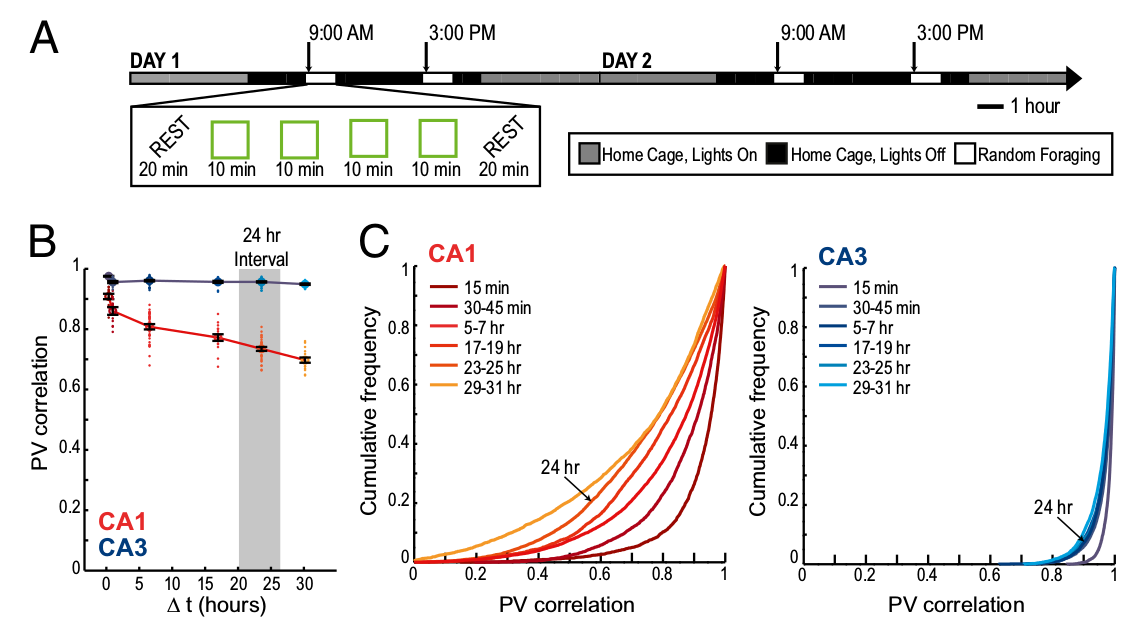
\includegraphics[width=0.8\textwidth]{intro/Mankin2012}
	\caption[Place cell population stability over days]{
		When testing with a single enclosure shape, firing patterns of the CA3 network remained highly consistent for repetitions of the same environment over extended time intervals, whereas activity patterns in the CA1 network changed.
		(A) An experimental design with a single enclosure shape.
		(B) PV correlations between pairs of recordings are shown as dots. The black error bars report the mean $\pm$ SEM for pair-wise comparisons at each time interval.
		% The correlation coefficients for the CA1 population activity (red) decreased monotonically as a function of elapsed time between recording sessions up to at least 30~h.
		Highly consistent firing patterns in the CA3 population were observed over time intervals of 30~min to 30~h. In contrast, the CA1 network continued to show a pronounced monotonic decrease in firing similarity with time.
		(C) Cumulative distribution functions for PV correlations between pairs of recordings at different time intervals
	Reproduced from \citet{Mankin2012}.}
	\label{fig:intro:memory:time_stability}
\end{figure}

\todo{Include Kentros}
\citep{Thompson1990}